

Giganttinen web-palvelin, joka hoitaa Kaiken tällä hetkellä.

LDAP, jossa käyttäjät, integroitu web-palveluihin.

halutaan olla SOA.

Sikteeri on Kapsin jäsenrekisteri ja laskutusohjelmisto. Tämä täytyisi selittää auki tekstissä, koska se on oleellisin juttu kokonaisuden kannalta.


\begin{figure}[h]
\centering
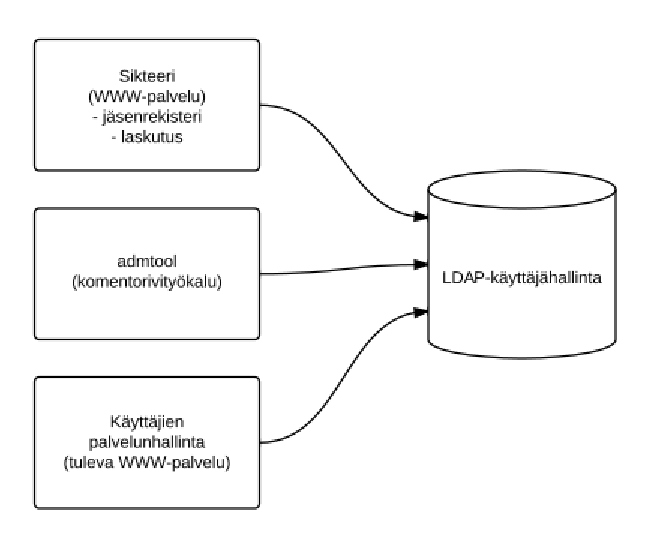
\includegraphics[width=.7\textwidth]{toteutus/kapsi_nykyinen.eps}
\caption{Kapsin jäsenhallintapalveluiden arkkitehtuuri. Sikteerin lisäksi arkkitehtuuriin kuuluu tietokanta ja käyttäjähallinta.}%
\label{kapsi_nykyinen}
\end{figure}

\begin{figure}[h]
\centering
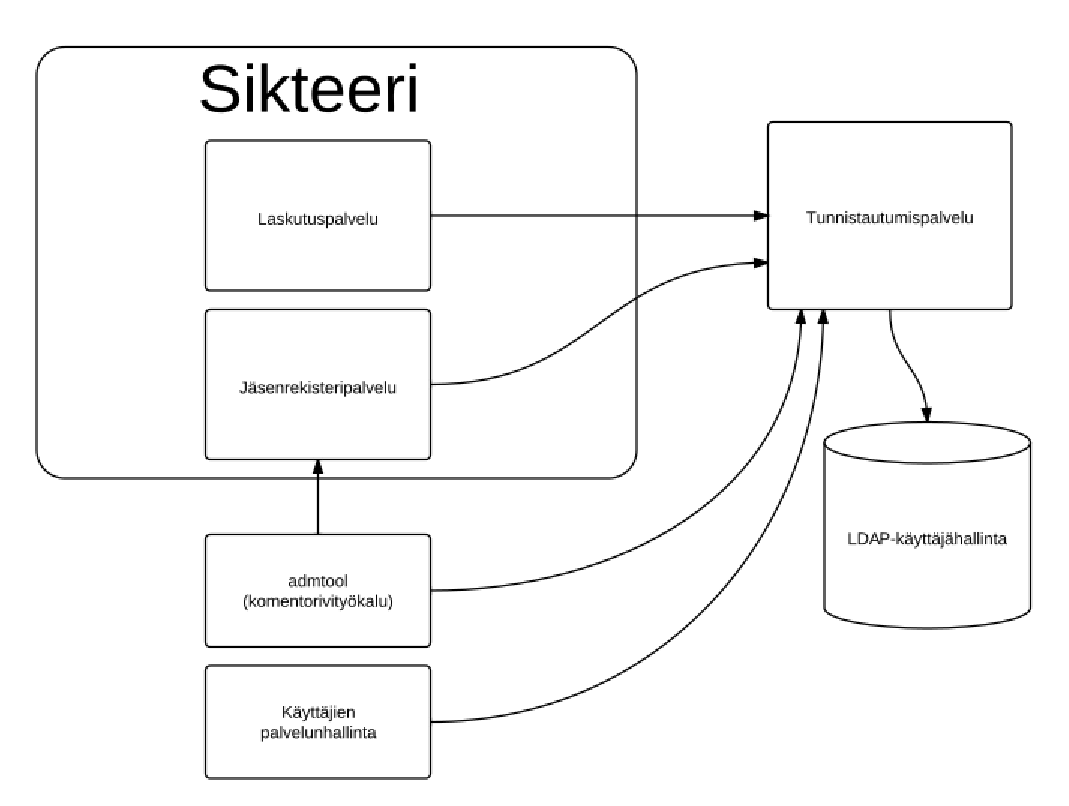
\includegraphics[width=.7\textwidth]{toteutus/kapsi_uusi.eps}
\caption{Palvelusuuntautuneen arkkitehtuurin mukainen kuvaus Kapsin järjestelmästä. Sikteerin palvelut on jaoteltu omiksi komponenteiksi ja järjestelmään on lisätty keskitetty tunnistautumispalvelu.}%
\label{kapsi_uusi}
\end{figure}